% use "pdflatex" engine

\documentclass[11pt, a4paper]{article}

\usepackage{type1cm} % allow all font size???
\usepackage{amsfonts, amssymb, amsmath} % for "align*"
\usepackage{fancyhdr} \setlength{\headheight}{13.69999pt}
\usepackage{enumerate}

% Require "texlive-latex-extra" package in your device. Use apt.
\usepackage{tikz}
\usetikzlibrary{shapes.geometric, arrows}

\usepackage{hyperref} % Solve the conflict between "tikz" and "tableofcontent"

% declares

%% flowchart

\tikzstyle{startstop} = [rectangle, rounded corners, minimum width = 3cm,
  minimum height = 1cm, text centered, draw = black, fill = red!30]
\tikzstyle{io} = [trapezium, trapezium left angle = 60, trapezium right angle =
  120, minimum width = 3cm, minimum height = 1cm, text centered, draw = black,
  fill = blue!30]
\tikzstyle{decision} = [diamond, minimum width = 3cm, minimum height = 1cm, text
centered, draw = black, fill = green!30]
\tikzstyle{process} = [rectangle, minimum width = 3cm, minimum height = 1cm,
  text centered, draw = black, fill = orange!30]
\tikzstyle{arrow} = [thick, ->, >=stealth]

\title{ \LaTeX\ }
\author{author}
% \date{January 1, 1970}
\date{\today}

\begin{document}

\maketitle
\thispagestyle{empty}
\pagebreak

\pagenumbering{roman}
\setcounter{page}{1}
\tableofcontents
\pagebreak
\pagenumbering{arabic}
\setcounter{page}{1}

\pagestyle{fancy}
\fancyhead[L]{ \LaTeX\ }
\fancyhead[R]{\nouppercase{\leftmark}}

ection{Creating a \LaTeX\ Document}
llo! This is my first \LaTeX\ document.

rectangle has side lengths of $(x + 1)$ and $(x + 3)$.
e equation $${A(x) = x^2 + 4x + 3}$$ gives the area of the rectangle.

\section{Common Mathematical Notation}

\subsection{Superscripts}

$$ 2x^{3x^{4x^{5x+6}}} $$

\subsection{Subscripts}

$$ 2x_{3x_{4x_{5x+6}}} $$
$$ a_0, a_1, a_2, \ldots, a_{100} $$

\subsection{Greek Letters}

$$ \pi $$
$$ \Pi $$
$$ \alpha $$
$$ A = \pi r^2 $$

\subsection{Trig Functions}

$$ y = \sin x $$
$$ y = \cos x $$
$$ y = \csc \theta $$

\subsection{Log Functions}

$$ \ln x = \log_e x $$

\subsection{Roots}

$$ \sqrt{x} = \sqrt[2]{x} $$

\subsection{Fractions}

$$ \frac{2}{3} $$
About $\displaystyle \frac{2}{3}$ of the glass is full.\\
About $\frac{2}{3}$ of the glass is full.

\section{Brackets, Tables, and Arrays}

\subsection{Brackets}

The distributive property states that $a(b + c) = ab + ac$, for all $a, b, c \in \mathbb{R}$. The equivalence class of $a$ is $[a]$.\\
The set $A$ is defined to be $\{1, 2, 3\}$.\\
The movie ticket costs $\$11.50$.
$$ 2 \left( \frac{1}{x^2 + 1} \right) $$
$$ 2 \left\langle \frac{1}{x^2 + 1} \right\rangle $$
$$ 2 \left| \frac{1}{x^2 + 1} \right| $$
$$ \left. \frac{dy}{dx} \right|_{x = 1} $$

\subsection{Tables}

\begin{table}[ht]
  \centering
  \begin{tabular}{|c||c|c|c|c|c|}       \hline
      $x$  &  1 &  2 &  3 &  4 &  5  \\ \hline
    $f(x)$ & 10 & 11 & 12 & 13 & 14  \\ \hline
  \end{tabular}
  \caption{These values represent the function $f(x)$.}
\end{table}
\begin{table}[ht]
  \def \arraystretch{1.2}
  \caption{These values represent the function $f(x)$.}
  \begin{tabular}{|c||c|c|c|c|c|}       \hline
      $x$  &  1 &  2 &  3 &  4 &  5  \\ \hline
    $f(x)$ & 10 & 11 & 12 & 13 & 14  \\ \hline
  \end{tabular}
\end{table}

\subsection{Arrays}
\begin{align}
       5x^2 - 9 &= x + 3\\
  5x^2 - x - 12 &= 0
\end{align}

\section{Creating Lists}

\subsection{Enumerate}

\begin{enumerate}[A.]
\item pencil
\item calculator
\item ruler
\item notebook
  \begin{enumerate}
  \item notes
  \item homework
  \item assessments
  \end{enumerate}
\item highlighter
\end{enumerate}

\subsection{Itemize}

\begin{itemize}
\item pencil
\item calculator
\item ruler
\item notebook
  \begin{itemize}
  \item notes
  \item homework
  \item assessments
  \end{itemize}
\item highlighter
\end{itemize}

\section{Text Document Formatting}

This will produce \textit{italicizd} text.

This will produce \textbf{bold face} text.

This will produce \textsc{small caps} text.

This will produce \texttt{typewriter font} text.

\begin{tiny}+tiny+\end{tiny}
\begin{scriptsize}+scriptsize+\end{scriptsize}
\begin{small}+small+\end{small}
\begin{normalsize}+normalsize+\end{normalsize}

\begin{normalsize}+normalsize+\end{normalsize}
\begin{large}+large+\end{large}
\begin{Large}+Large+\end{Large}
\begin{huge}+huge+\end{huge}
\begin{Huge}+Huge+\end{Huge}

\begin{flushleft}
  flushleft
\end{flushleft}

\begin{center}
  center
\end{center}

\begin{flushright}
  flushright
\end{flushright}

\section {Flowchart}

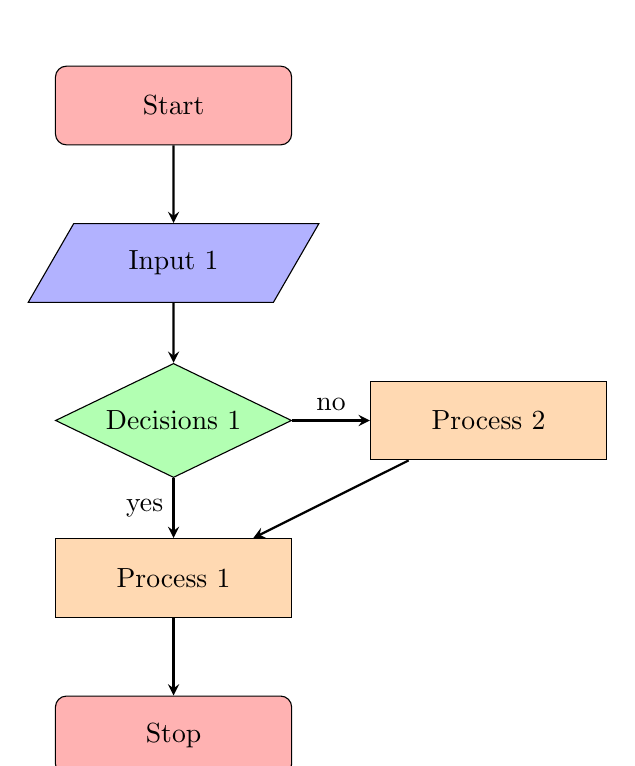
\begin{tikzpicture}[node distance = 2cm]
  \node (start) [startstop] {Start};
  \node (input-1) [io, below of = start] {Input 1};
  \node (decision-1) [decision, below of = input-1, aspect = 2] {Decisions 1};
  \node (process-1) [process, below of = decision-1] {Process 1};
  \node (process-2) [process, right of = decision-1, xshift = 2cm] {Process 2};
  \node (stop) [startstop, below of = process-1] {Stop};

  \draw [arrow] (start) -- (input-1);
  \draw [arrow] (input-1) -- (decision-1);
  \draw [arrow] (decision-1) -- node[anchor = east] {yes} (process-1);
  \draw [arrow] (decision-1) -- node[anchor = south] {no} (process-2);
  \draw [arrow] (process-2) -- (process-1);
  \draw [arrow] (process-1) -- (stop);
\end{tikzpicture}

\end{document}
